\section{Обходы графов. Обход в ширину, обход в глубину. }

\subsection*{Обход графа}
\textbf{Обход графа} --- способ однократного просмотра всех вершин связного графа в определённом порядке. 
Обход всегда начинается с заданной вершины. 
Важно, чтобы каждая вершина была просмотрена и притом только один раз.

\subsection*{Обход в ширину (BFS)}
Пусть задан граф $G=(V,E)$, выделена исходная вершина $s$. 
Алгоритм обходит все рёбра для "открытия" всех вершин, достижимых из $s$, вычисляя при этом расстояние от $s$ до каждой открытой вершины.
\begin{itemize}
	\item Изначально все вершины белые.
	\item Когда вершина впервые открыта, красим её в серый.
	\item Если $(u,v) \in E$ и, если $u$ чёрная, то $u$ либо чёрная, либо серая.
	\item Все вершины, смежные с чёрной, уже открыты.
	\item Серые вершины могут иметь белых соседей.
	\item В процессе обхода строится дерево поиска в ширину с корнем $s$, содержащее все посещённые вершины.
\end{itemize}

\subsubsection*{Алгоритм:}
\begin{enumerate}
	\item Из графа выбирается первая вершина и помечается, как посещённая, заносясь в очередь.
	\item Посещается одна вершина из начала очереди, если она не помечена как посещённая. Все её соседние непосещённые вершины заносятся в очередь и в дерево, а сама она из неё удаляется.
	\item Повторяется п.2, пока очередь не опустеет.
\end{enumerate}
\begin{figure}[h!]
	\centering
	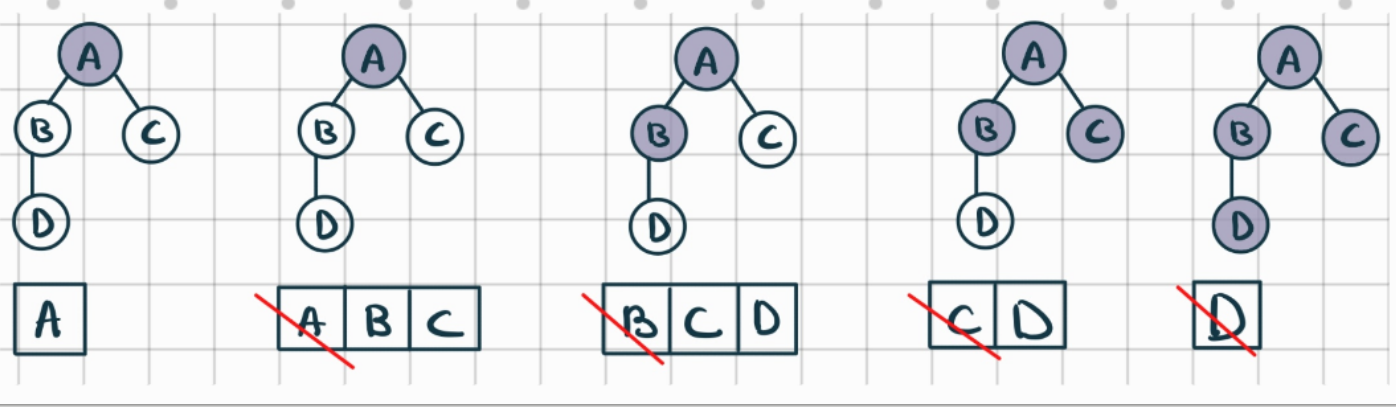
\includegraphics[width=0.6\linewidth]{img_easy/6_1.png}
	\captionsetup{labelformat=empty}
	\caption{Пример работы поиска в ширину}
	\label{fig:51}
\end{figure}

\subsubsection*{Лемма:}
В очереди поиска в ширину расстояние от вершины до $s$ монотонно неубывает.

\subsubsection*{Теорема:}
Алгоритм поиска в ширину в невзвешенном графе находит длины кратчайших путей до всех достижимых вершин.
(находит в неориентированном графе кратчайший путь по количеству рёбер)

\subsubsection*{Доказательство:}
Допустим, что это не так. Выберем из вершин, для которых кратчайший путь от $s$ найден некорректно, ту, настоящее расстояние до которой $min$. Пусть это вершина $u$, её предок в дереве обхода --- вершина $v$, а предок в кратчайшем пути --- вершина $w$.
Т.к. $w$ --- предок в кратчайшем пути, то $\rho(s,u)=\rho(s,w)+1 > \rho(s,w)$. 
И расстояние до $w$ найдено верно $\rho(s,w)=d[w] \implies \rho(s,u)=d[w]+1$.
Т.к. $v$ --- предок в дереве обхода в BFS: $d[u]=d[v]+1$. 
Расстояние до $u$ найдено некорректно $\implies \rho(s,u) < d[u]$.
$\implies d[w]+1 < d[v]+1 \implies d[w] < d[v]$.
По лемме в этом случае вершина $w$ попала в очередь и была обработана раньше, чем $v$. Но $w$ не может быть предком $u$ в дереве обхода в ширину --- противоречие.

\subsubsection*{Анализ времени работы:}
В очередь добавляются только непосещённые вершины $\implies$ каждая вершина посещается не более 1 раза.
Операции внесения в очередь и удаления --- $O(1)$ $\implies$ общее время работы с очередью $O(V)$.
Для каждой вершины рассматривается не более $deg(v)$ рёбер, инцидентных ей.
Т. к. $\sum deg(v) = 2|E|$ $\implies$ время на работу с рёбрами $O(E)$.
Общее время работы: $O(V+E)$. 
\begin{observation}
	$O(V + E)$ получается только при реализации графа на списках смежности и CSR --- при представлении графа на матрице смежности оценка $O(V^2)$
\end{observation}

\subsection*{Обход в глубину (DFS)}
Исследуются все рёбра графа, исходящие из вершины, открытой последней, и покидает её только тогда, когда не осталось неисследованных рёбер. 
Происходит "откат" в вершину, из которой была открыта вершина $v$. Процесс повторяется, пока не будут открыты все вершины.

\subsubsection*{Алгоритм:}
\begin{enumerate}
	\item Выбирается начальная вершина, отмечается как посещённая и заносится в стек.
	\item В стеке находится последняя посещённая вершина. Для неё выбирается первая непосещённая вершина и ей присваивается значение "посещение" и добавляется в стек (рекурсивный вызов функции для соседних с последней вершиной в стеке).
	\item Если таких вершин нет, то она удаляется из стека, и процесс повторяется для предыдущей вершины.
	\item Повторять 1, 2 и 3, пока стек не станет пустым.
\end{enumerate}

\subsubsection*{Анализ времени работы:}
Процедура DFS вызывается от каждой вершины не более 1 раза.
Внутри процедуры рассматриваются все такие рёбра $\{e \mid begin(e)=u\}$.
Всего таких рёбер для всех вершин в графе $O(E)$ $\implies$ время работы алгоритма $O(V+E)$.

\begin{observation}
	Аналогично поиску в ширину, $O(V + E)$ получается только при реализации графа на списках смежности и CSR --- при представлении графа на матрице смежности оценка $O(V^2)$
\end{observation}
